\section{Analytic form of Hahn-Banach: Extensions of linear functionals}
\subsection{Extensions of linear functionals}
\begin{definition}\label{iv.1}
    Let $X$ be a vector space. A map $\func{p}{X}{\R}$ is \bol{sublinear}\index{sublinear} if
    \begin{enumerate}[label=\alph*)]
        \item $p(\lambda x)=\lambda p(x)\;\;\;\forall\lambda\geq0,x\in X$.
        \item $p(x_1+x_2)\leq p(x_1)+p(x_2)\;\;\;\forall x_1,x_2\in X$.
    \end{enumerate}
\end{definition}

\paragraph{Examples}
\begin{enumerate}[label=\arabic*)]
    \item Every seminorm on $X$ is sublinear.
    \item Every linear functional on a real vector space is sublinear (it is even linear).
    \item On $\ell^\infty(\N,\R)$ the map
        \[\ell^\infty(\N,\R)\ni (t_n)_n\mapsto\limsupn t_n\]
        is sublinear. On $\ell^\infty(\N,\C)$ the maps
        \[t=(t_n)_n\mapsto\limsupn\RE(t_n)\te{ and }t=(t_n)_n\mapsto\limsupn|t_n|\]
        are sublinear.
    \item Sublinear functions are often called Minkowski functionals.
\end{enumerate}

\begin{thm}[Hahn-Banach, analytic form]\label{iv.2}\index{Hahn-Banach!analytic form}
    Let $E$ be a real vector space, $\func{p}{E}{\R}$ sublinear. Given a linear subspace $A\subset E$ \rec{(}i.e. $A$ is a vector subspace of $E$\rec{)} and $\func{g}{A}{\R}$ a linear functional with
    \[g(x)\leq p(x)\;\;\;\forall x\in A\tag{4.1}\label{4.1}\]
    there exists a linear functional $\func{\ell}{E}{\R}$ which extends $g$ \rec{(}that is, $\ell(x)=g(x)\;\;\forall x\in A$\rec{)} such that also
    \[\ell(x)\leq p(x)\;\;\;\forall x\in E.\tag{4.2}\label{4.2}\]
\end{thm}

\begin{cor}\label{iv.3}
    Let $E$ be a real normed vector space with norm $\|\cdot\|_E$. Then for all $x\in E$
    \[\|x\|_E=\sup_{\substack{\ell\in E^*\\\|\ell\|_{E^*}\leq 1}}\ell(x)=\sup_{\substack{\ell\in E^*\\\|\ell\|_{E^*}\leq 1}}|\ell(x)|.\tag{4.8}\label{4.8}\]
    In particular, for $x_1\neq x_2\in E$, there exists $\ell\in E^*$ with $\|\ell\|_{E^*}=1$ and $\ell(x_1)\neq\ell(x_2)$, i.e., $E^*$ separates the points in $E$.
\end{cor}

\subsection{Complexification of the Hahn-Banach extension theorem}
\rec{Situation:} We are given a complex vector space $E$ with a sublinear function $\func{p}{E}{\R}$ (i.e., $p(\lambda x)=\lambda p(x)\;\forall x\in E,\lambda\geq0$ and $p(x_1+x_2)\leq p(x_1)+p(x_2)$) and a subspace $A\subset E$ and a linear functional $\func{g}{A}{\C}$ with
\[\RE g(x)\leq p(x)\;\;\;\forall x\in A.\tag{4.12}\label{4.12}\]
We have to take the real part in \eqref{4.12}. since $g$ is complex valued.

\begin{lem}\label{iv.4}
    Let $E$ be a $\C$-vector space
    \begin{enumerate}[label=\alph*)]
        \item If $\func{h}{E}{\R}$ is real linear, i.e. $h(\alpha x_1+\beta x_2)=\alpha h(x_1)+\beta h(x_2)$ for all $x_1,x_2\in E,\alpha,\beta\in\R$, then $\func{h_\C}{E}{\C}$ defined by 
        \[h_\C(x):=h(x)-\mathrm{i}h(\mathrm{i}x),\;\;x\in E\]
        defines a complex linear functional with $h=\RE h_\C$.\label{iv.4.a}
        \item If $\func{\ell}{E}{\C}$ is complex linear, then $h:=\RE\ell$ is real linear and $\ell=h_\C$.\label{iv.4.b}
        \item If $\func{p}{E}{\C}$ is sublinear and symmetric, that is, $p(ax)=p(x)$ for all $x\in E$ and $a\in \C$ with $|a|=1$, and $\func{\ell}{E}{\C}$ is complex linear, then
        \[|\ell(x)|\leq p(x)\;\;\;\forall x\in E\;\Lolrarr\;\RE\ell(x)\leq p(x)\;\;\;\forall x\in E.\tag{4.18}\label{4.18}\]\label{iv.4.c}
        \item If $\|\cdot\|$ is a norm on $E$ and $\ell\in E^*=L(E,\C)=$ bounded continuous complex valued linear functionals, then $\RE\ell\in L(E,\R)$ \rec{(}where for $L(E,\R)$, we consider $E$ as a real normed vector space\rec{)} and
        \[\|\ell\|_{L(E,\C)}=\|\RE\ell\;\|_{L(E,\R)}.\tag{4.19}\label{4.19}\]\label{iv.4.d}
    \end{enumerate}
\end{lem}

\begin{thm}[Hahn-Banach, complex form]\label{iv.5}\index{Hahn-Banach!complex form}
    Let $E$ be a complex vector space, $A\subset E$ a sub vector space, $\func{p}{E}{\R}$ sublinear and $\func{g}{A}{\C}\te{ complex linear with}$
    \[\RE g(x)\leq p(x)\;\;\;\forall x\in A. \tag{4.20}\label{4.20}\]
    Then there exists a complex linear map $\func{\ell}{E}{\C}$ which extends $g$ and 
    \[\RE\ell(x)\leq p(x)\;\;\;\forall x\in E.\tag{4.21}\label{4.21}\]
\end{thm}

\paragraph{Remark}
Instead of \eqref{4.20} we can also assume only that $A\subset E$ is a real sub vector space of $E$ and $\func{g}{A}{\R}$ is real linear and $g(x)\leq p(x)\;\;\;\forall x\in A$. 

Then there exists a complex linear map $\func{\ell}{E}{\C}$ with $\RE\ell(x)=g(x)\;\;\;\forall x\in A$ and $\RE\ell(x)\leq p(x)\;\;\;\forall x\in E$.

\begin{cor}\label{iv.6}
    Let $\K=\R$ or $\C$ and $E$ a normed $\K$-vector space and $A\subset E$ a linear subspace. Then for any $g\in L(A,\K)=A^*$ there exists an extension $\ell\in E^*=L(E,\K)$ of $g$ \rec{(}i.e., $\ell(x)=g(x)\;\;\;\forall x\in A$\rec{)} with
    \[\|\ell\|_{E^*}=\|g\|_{A^*}.\tag{4.22}\label{4.22}\]
\end{cor}

\begin{cor}\label{iv.7}
    Let $E$ be a complex normed vector space with norm $\|\cdot\|_E$. Then
    \[\|x\|_E=\sup_{\substack{\ell\in E^*\\\|\ell\|_{E^*}\leq1}}\RE\ell(x)=\sup_{\substack{\ell\in E^*\\\|\ell\|_{E^*}\leq1}}|\ell(x)|\tag{4.23}\label{4.23}\]
    for every $x\in E$.
\end{cor}

\begin{cor}\label{iv.8}
    Let $E$ be a normed vector space \rec{(}real or complex\rec{)} and $A\subsetneqq E$ be a closed subspace. Then for any $x_0\in E\setminus A$ there exists $\ell\in E^*$ such that $\ell(x_0)\neq0$ and $\ell(y)=0$ for every $y\in A$.
\end{cor}

\begin{definition}\label{iv.9}\ 
    \begin{enumerate}[label=\alph*)]
        \item Let $E$ be a Banach space and $A$ a closed subspace. We say that $w_1,\ldots,w_n\in E$ are \bol{independent over $A$} if $\sum_{j=1}^n\lambda_jw_j\in A$, $\lambda_j\in\K,j=1,\ldots,n$ implies $\lambda_j=0$, $j=1,\ldots,n$.\label{iv.9.a}
        \item The \bol{codimension} of $A$, $\rec{codim}(A)$ is given by
        \[\sup\big\{m\in \N\colon w_1,\ldots,w_m\!\te{\! are\! independent\! over }\!A\!\te{ for\! some\! choice\! of }m\!\te{ vectors\! }w_j\in E,\,j=1,\ldots,m\big\}.\]
    \end{enumerate}
\end{definition}

\begin{thm}\label{iv.10}
    Let $E$ be a Banach space and $A$ a closed subspace. Then
    \[\rec{codim}(A)=\dim\big\{\ell\in E^*\colon\ell|_A=0\big\}.\tag{4.25}\label{4.25}\]
\end{thm}

\subsection{Geometric forms of the Hahn-Banach theorems}
\begin{definition}\label{iv.11}
    An \bol{affine hyperplane}\index{affine hyperplane} is a subset $H$ of $E$ of the form
    \[H=\{x\in E\colon\RE \ell(x)=\alpha\}\tag{4.27}\label{4.27}\]
    where $\func{\ell}{E}{\K}$ is a linear functional which does not vanish identically on $E$ and $\alpha\in\R$.
    
    We write $H=[\RE\ell=\alpha]$ and call $\RE\ell=\alpha$ the \bol{equation for $H$}.
\end{definition}

\begin{lem}\label{iv.12}
    The hyperplane $H$ is closed iff $\ell$ is continuous \rec{(}i.e., $\ell\in E^*$\rec{)}.
\end{lem}

\begin{definition}\label{iv.13}
    Let $A,B\subset E$ be subsets of $E$. Then the hyperplane $H=[\RE\ell=\alpha]$ \bol{separates $A$ and $B$}\index{separate} if
    \[\RE\ell(x)\leq\alpha\;\;\forall x\in A\te{ and }\RE\ell(y)\geq\alpha\;\;\forall y\in B.\tag{4.31}\label{4.31}\]
    picture:
    \begin{figure}[!h]
        \centering
        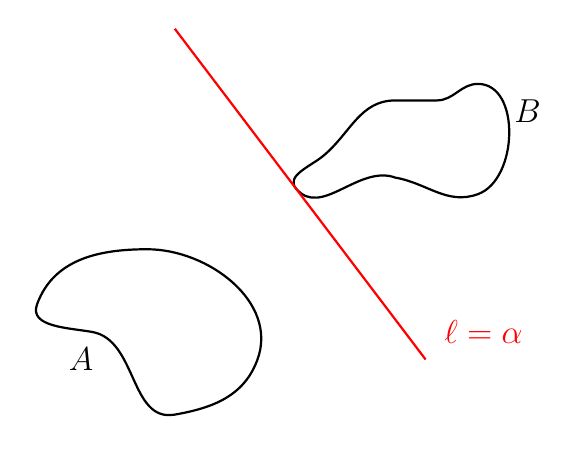
\begin{tikzpicture}[scale=0.7]
        %		A
        \node at (-4.2,-2){\large$A$};
        \draw[thick] (-3,0) to[out=0,in=70] (-1,-2) to[out=250,in=10] (-2.5,-3) to[in=350,out=190] (-4,-1.5) to[in=250,out=170](-5,-1) to[out=70,in=180] (-3,0);
        
        %		B
        \draw[thick] (3,3) to[out=0,in=20] (3,1) to[out=200,in=350] (1.5,1.3) to[out=160,in=310] (-0.3,1.1) to[out=130,in=220] (0.2,1.7) to[out=40,in=180] (1.5,2.7) to[out=0,in=180] (2.25,2.7) to[out=0,in=180] (3,3);
        \node at (3.9,2.5){\large$B$};
        
        %		slope
        \draw[thick,red] (-2.5,4)--(2.05,-2);
        \node[red] at (3.1,-1.5){\large$\RE\ell=\alpha$};
        \end{tikzpicture}%}\\
    \end{figure}\\
    
    We say that the separation is \bol{proper}\index{separate!properly} if $(A\cup B)\setminus H\neq\emptyset$ \rec{(}i.e., not both $A$ and $B$ are in the same halfplane \rec{(}i.e., we do not have $A\subset H$ and $B\subset H$\rec{)}\rec{)}.
    
    The hyperplane $H=[\RE\ell=\alpha]$ \bol{strictly separates}\index{separate!strictly} $A$ and $B$ if it separates them and
    \[\RE\ell(x)\neq\RE\ell(y)\;\;\;\forall x\in A,y\in B\tag{4.32}\label{4.32}\]
    and it \bol{strongly separates}\index{separate!strongly} $A$ and $B$ if there exists an $\varepsilon>0$ such that
    \[\RE\ell(x)\leq\alpha-\varepsilon\;\;\;\forall x\in A\te{ and }\RE\ell(x)\geq\alpha+\varepsilon\;\;\;\forall x\in B.\tag{4.33}\label{4.33}\]
    So $A$ and $B$ are separated with a safety distance.
\end{definition}

\begin{thm}[Hahn-Banach, first geometric form]\label{iv.14}\index{Hahn-Banach!first geometric form}
    Let $E$ be a normed vector space and $\emptyset\neq A,B\subset E$ disjoint, convex subsets of $E$ such that one of them has an interior point. Then there exists a closed hyperplane $H$ which properly separates them.
\end{thm}

\begin{definition}\label{iv.15}
    Let $E$ be a vector space and $A\subset E$. Then the \bol{Minkowski gauge}\index{Minkowski gauge} $p_A$ is given by
    \[p_A(x):=\inf\{\lambda>0\colon\lambda^{-1}x\in A\}\tag{4.34}\label{4.34}\]
    with convention that $\inf\emptyset:=\infty$. 
    
    So $p_A(x)=\infty\Lolrarr$ For no $\lambda>0$ does one have $\lambda^{-1}x\in A$.
\end{definition}

\begin{definition}\label{iv.16}
    A function $\func{p}{E}{[0,\infty)}$ is \bol{positive homogenous of degree 1} \rec{(}or for short, \bol{homogenous}\rec{)} if
    \[p(\lambda x)=\lambda p(x)\;\;\;\forall x\in E,\lambda\geq0.\]
\end{definition}

\begin{prop}\label{iv.17}
    Let $E$ be a $\K$-vectorspace and $\func{p}{E}{[0,\infty)}$ homogenous. Then the statements
    \begin{enumerate}[label=\alph*)]
        \item \rec{(}Triangle inequality\rec{)}\label{iv.17.a}
        \[p(x+y)\leq p(x)+p(y)\;\;\;\forall x,y\in E.\tag{4.35}\label{4.35}\]
        
        \item \rec{(}Convexity of $p$\rec{)} $p$ is a convex function, that is,\label{iv.17.b}
        \[p((1-\theta)x+\theta y)\leq(1-\theta)p(x)+\theta p(y)\;\;\;\forall x,y\in E,0\leq\theta\leq1.\tag{4.36}\label{4.36}\]
        
        \item \rec{(}Convexity of the unit ball \rec{(}given by $p$\rec{)}\rec{)}\label{iv.17.c}
        \[B_p:=\{x\in E\colon p(x)\leq1\}\te{ or }\widetilde{B}_p:=\{x\in E\colon p(x)<1\}\]
        is convex. 
    \end{enumerate}
    are equivalent.
\end{prop}

\begin{definition}\label{iv.18}
    Let $E$ be a real or complex vector space. A set $A\subset E$ is called \bol{absorbing}\index{absorbing} if
    \[0\in A\te{ and }E=\cupp_{\lambda>0}\lambda A.\tag{4.38}\label{4.38}\]
    It is called \bol{pseudo-open}\index{pseudo-open} if for any $x\in A$ and any $y\in E$, there exists $\delta_0>0$ such that $x+\alpha y\in A\;\;\forall|\alpha|<\delta_0$. $A$ is called \bol{balanced}\index{balanced} if
    \[x\in A\te{ and }\alpha\in\K,|\alpha|=1\te{ implies }\alpha x\in A.\tag{4.39}\label{4.39}\]
\end{definition}

\begin{prop}\label{iv.19}
    Let $E$ be a real or complex vector space and $A$ a convex, absorbing subset of $E$. Define the Minkowski gauge
    \[p_A(x):=\inf\{\lambda>0\colon\lambda^{-1}x\in A\}\]
    of $A$. Then
    \begin{enumerate}[label=\alph*)]
        \item $\func{p_A}{E}{[0,\infty)}$ is a homogenous, convex function with\label{iv.19.a}
        \[\{p_A<1\}\subset A\subset \{p_A\leq1\}\tag{4.40}\label{4.40}\]
        \big(We set $\{p_A<1\}=\{x\in E\colon p_A(x)<1\}$ etc.\big)
        \item If $A$ is pseudo-open, then\label{iv.19.b}
        \[A=\{p_A<1\}.\tag{4.41}\label{4.41}\]
        \item If $A$ is balanced, then $p_A$ is a seminorm.\label{iv.19.c}
        \item If $E$ is a normed vector space and $A\subset E$ is convex and zero is in the interior of $A$ \big(i.e., $\exists r>0\colon B_r(0)=\{x\in E\colon\|x\|_E<r\}\subset A$\big) then there exists $M<\infty$ such that\label{iv.19.d}
        \[p_A(x)\leq M\|x\|_E\;\;\;\forall x\in E.\tag{4.42}\label{4.42}\]
        \item If $A$ contains a subspace $B$ of $E$ then\label{iv.19.e}
        \[p_A(x)=0\;\;\;\forall x\in B.\tag{4.43}\label{4.43}\]
    \end{enumerate}
\end{prop}

\begin{lem}\label{iv.20}
    Let $E$ be a $\K$-vector space and $\emptyset\neq C\subset E$ convex and assume that $0$ is an interior point of $C$ and $x_0\notin C$. Then there exists $\ell\in E^*$ such that
    \begin{equation}
    \tag{4.44}\label{4.44}
        \begin{aligned}
        \RE\ell(x)&\leq p_C(x)\;\;\;\forall x\in E,\\
        \RE\ell(x)&\leq p_C(x_0)\;\;\;\forall x\in C,\\
        \RE\ell(x_0)&=p_C(x_0)\geq1,
        \end{aligned}
    \end{equation}
    where $p_C$ is the Minkowski gauge of $C$.
\end{lem}

\begin{thm}[Hahn-Banach, second geometric form]\label{iv.21}\index{Hahn-Banach!second geometric form}
    Let $E$ be a normed vector space and $\emptyset\neq A,B\subset E$ disjoint, convex subsets of $E$ such that one of them is open. Then there exists a closed hyperplane $H$ which strictly separates them.
\end{thm}

\begin{thm}[Hahn-Banach, third geometric form]\label{iv.22}\index{Hahn-Banach!third geometric form}
    Let $E$ be a normed vector space and $\emptyset\neq A,B\subset E$  convex, disjoint and assume that $A$ is closed and $B$ is compact. Then there exists a closed hyperplane which strongly separates them.
\end{thm}

\begin{definition}\label{iv.23}
    The \bol{bidual}\index{bidual} $E^{**}$ is the dual of $E^*$ that is, $E^{**}=(E^*)^*=L(E^*,\K)$ with norm
    \[\|\xi\|_{E^{**}}=\sup_{\substack{\ell\in E^*\\\|\ell\|_{E^*}\leq1}}|\xi(\ell)|,\;\;\;\xi\in E^{**}.\tag{4.49}\label{4.49}\]
\end{definition}
Note that every $x\in E$ can be identified with an element $\xi_x\in E^{**}$ by setting
\[\xi_x(\ell):=\ell(x). \tag{4.50}\label{4.50}\]
since $E^*\ni\ell\mapsto\ell(x)$ is, for fixed $x\in E$, 
a continuous linear functional on $E^*$. 
Thus there is a canonical injection $\func{J}{E}{E^{**}}$, 
$x\mapsto J(x):=\xi_x$ (as in \eqref{4.50}) so 
$J(x)(\ell)=\xi_x(\ell)=\ell(x)\;\;\forall\ell\in E^*$.

\paragraph{Notation:}
If $M\subset E$ is a linear subset, we set
\[M^\perp:=\{\ell\in E^*\colon\ell(x)=0\;\;\forall x\in M\}.\tag{4.52}\label{4.52}\]
If $N\subset E^*$, then we set
\[N^\perp:=\{x\in E\colon\ell(x)=0\;\;\forall\ell\in N\}.\tag{4.53}\label{4.53}\]
Note that, by definition, $N^\perp\subset E$. (not a subset of $E^{**}$)

It is clear, by continuity, that $M^\perp$, respectively $N^\perp$, 
is a closed subspace of $E^*$, respectively $E$. We say $M^\perp\subset E^*$ is 
\rec{\bol{orthogonal}} to $M\subset E$ and $N^\perp\subset E$ is \rec{\bol{orthogonal}} 
to $N\subset E^*$.

\begin{prop}\label{iv.24}
    Let $M\subset E$ be a linear subspace, then 
    \[(M^\perp)^\perp=\overline{M}.\tag{4.54}\label{4.54}\]
    Let $N\subset E^*$ be a linear subspace then
    \[(N^\perp)^\perp\supset\overline{N}.\tag{4.55}\label{4.55}\]
\end{prop}